\documentclass{article}
\usepackage[UTF8]{ctex}  % 使用中文支持包
\usepackage[a4paper, margin=1in]{geometry}  % 设置纸张大小和边距
\usepackage{anyfontsize}  % 解决字体大小报错问题
\usepackage{fancyhdr}  % 设置页眉、页脚、页码
\usepackage{longtable}  % 支持长表格

\usepackage{amsmath}  % 数学公式支持
\usepackage{cases}  % 支持联立编号

\usepackage{graphicx}  % 插入图片支持
\usepackage{float}  % 设置图片浮动位置
\usepackage{subfigure}  % 插入多图时用子图显示

\usepackage{listings}  % 代码块支持
\usepackage{xcolor}  % 设置代码块颜色

\usepackage[hyphens]{url}  % 支持链接换行
\usepackage{hyperref}  % 超链接支持
\usepackage{lastpage}  % 添加lastpage包
\usepackage{gbt7714}  %国标参考文献
\bibliographystyle{gbt7714-numerical}
\hypersetup{
    hidelinks,
    colorlinks=true,
    allcolors=black,
    pdfstartview=Fit,
    breaklinks=true
}

\title{射线源导论-第二周作业}
\author{\LaTeX\ by\ 何宇峰\ }
\date{\today}
\pagenumbering{arabic}

\begin{document}
\pagestyle{fancy}

\fancyhead[L]{何宇峰}
\fancyhead[C]{射线源导论-第三周作业}
\fancyhead[R]{\today}
\fancyfoot[C]{Page \thepage/\pageref{LastPage}}

\section*{第三周课程作业}

\subsection*{1. 重复Richardson-Dushman的推导过程}

由费米分布可知, 电子数密度与能量的函数关系为:

$$n(E) = g(E) f(E)$$

其中 $g(E) = \frac{4\sqrt{2}\pi g_s m^{\frac{3}{2}}\sqrt{E}}{h^3} = \frac{8\sqrt{2}\pi m^{\frac{3}{2}}\sqrt{E}}{h^3}$为电子态密度, 电子的自旋因子$g_s = 2s + 1 = 2 \times \frac{1}{2} + 1 = 2$, $f(E)=\frac{1}{1+e^{\frac{E-E_F}{kT}}}$是平均每个电子态的电子数.

故能量在$E$到$E+dE$之间的电子数为:

$$n(E)dE = \frac{8\sqrt{2}\pi m^{\frac{3}{2}}\sqrt{E}}{h^3} \frac{1}{1+e^{\frac{E-E_F}{kT}}}dE$$

考虑到$E_F$很小, 即$E \gg E_F $, 则有近似后的表达式

$$n(E)dE \approx \frac{8\sqrt{2}\pi m^{\frac{3}{2}}\sqrt{E}}{h^3} e^{- \frac{E-E_F}{kT}}dE = \frac{8\pi m^{3}\sqrt{E}}{h^3} e^{- \frac{\frac{1}{2}mv^2-E_F}{kT}}v^2dv$$

规定垂直于阴极面的方向为$x$方向, 只有$x$方向速度大于$v_{x.min} = \sqrt{\frac{2(W+E_F)}{m}}$的电子能够被发射, 则热发射的电流密度为:

\begin{equation*}
    \begin{aligned}
        J &= \int_{v_{x.min}}^{\infty} \text{e} n(v) v_x dv \\
        &= \int_{v_{x.min}}^{\infty} \text{e} v_x \frac{8\pi m^{3}\sqrt{E}}{h^3} e^{- \frac{\frac{1}{2}mv^2-E_F}{kT}}v^2dv \\
        &= \frac{2m^3\text{e}}{h^3} e^{\frac{E_f}{kT}} \int_{v_{x.min}}^{\infty} v_x e^{-\frac{mv^2}{2kT}}4\pi v^2 dv\\
        &= \frac{2m^3\text{e}}{h^3} e^{\frac{E_f}{kT}} \int_{v_{x.min}}^{\infty} v_x e^{-\frac{mv_x^2}{2kT}}\pi v_x^2 dv_x \int_{-\infty}^{\infty} e^{-\frac{mv_y^2}{2kT}}\pi v_y^2 dv_y \int_{-\infty}^{\infty} e^{-\frac{mv_z^2}{2kT}}\pi v_z^2 dv_z\\
        &= \frac{2m^3\text{e}}{h^3} e^{\frac{E_f}{kT}}\frac{kT}{m}e^{-\frac{m}{2kT}\frac{2(W+E_F)}{m}}\frac{2\pi kT}{m}\\
        &= \frac{4\pi m k^2 \text{e}}{h^3} T^2 e^{-\frac{W}{kT}}\\
        &= A T^2 e^{-\frac{W}{kT}}
    \end{aligned}
\end{equation*}

其中, $A = \frac{4\pi m k^2 \text{e}}{h^3}= 1.202 \times 10^6 \text{A}\text{m}^{-2}\text{K}^{-2}$. 实际中, $A$的大小随材料的不同而不同.

\subsection*{2. 如果对热阴极电流密度的稳定性要求优于1\%, 对其温度稳定性和功函数的变化分别有什么要求?}

$$ J = AT^2 e^{-\frac{W}{kT}}$$

则有

$$\frac{\partial J}{\partial T} = AT e^{-\frac{W}{kT}}\left(2+\frac{W}{kT}\right) = \frac{J}{T}(2+\frac{W}{kT})$$

$$\frac{\partial J}{\partial W} = -AT e^{-\frac{W}{kT}} = \frac{J}{kT}$$

对热阴极电流密度的稳定性要求优于1\%, 则有:

温度的稳定性应该满足 $$\frac{J}{T}(2+\frac{W}{kT})<1\%$$

故$$\left\lvert \frac{\Delta T}{T} \right\rvert <\frac{1\%}{2+\frac{W}{kT}}$$

功函数的变化应该满足: $$\frac{J}{kT}<1\%$$

故$$\left\lvert \frac{\Delta W}{W} \right\rvert <\frac{1\%}{\frac{W}{kT}}$$

\subsection*{3. 画出100-2000摄氏度(假设不熔化)铜、银、金、钨、LaB6的热发射电流密度}

$$J = A T^2 e^{-\frac{W}{kT}}$$

材料的功函数分别为: Cu: 4.65eV, Au: 5.10eV, Ag: 4.26eV, W: 4.55eV, LaB6: 2.70eV

热发射电流密度随温度变化的曲线如图\ref{fig:J-T}所示.

\begin{figure}[ht]
    \centering
    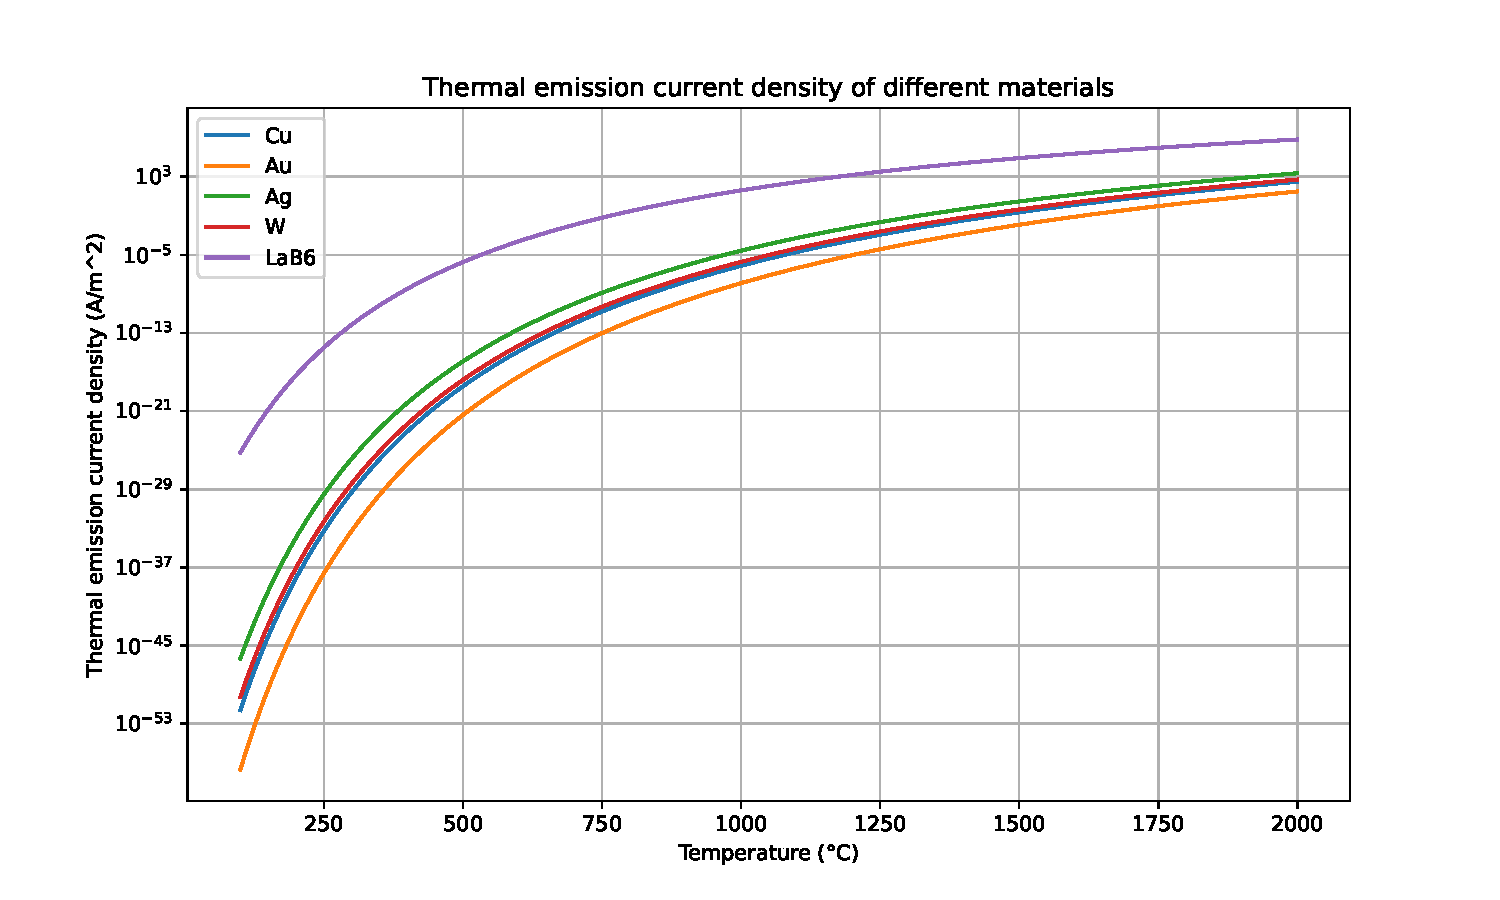
\includegraphics[width=0.7\textwidth]{img/J-T.pdf}
    \caption{热发射电流密度随温度变化}
    \label{fig:J-T}
\end{figure}

\subsection*{4. 基于热发射和光电发射的物理图像, 思考场致发射的原理}

场电子发射,也称为场发射(FE)和电子场发射,是指静电场诱导的电子发射. 最常见的情况是固体表面向真空的场发射. 然而,场发射也可以从固体或液体表面发生, 进入真空、流体(例如空气)或任何非导电或弱导电的绝缘体.\cite{Field-electron-emission}

在足够强的静电场中, 由于静电场所能提供的能量足够大, 材料中的电子可以克服材料的功函数(减少势垒大小), 更容易逸出材料表面, 从而产生场致发射.

\bibliography{cite.bib}

\end{document}
